\documentclass[tikz,border=2mm]{standalone}
\usepackage{pgfplots}
\pgfplotsset{compat=1.18}
\begin{document}

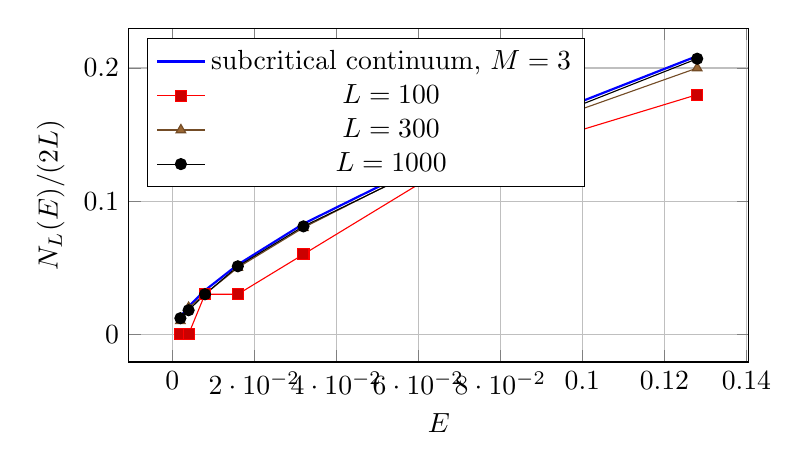
\begin{tikzpicture}
\begin{axis}[width=0.78\linewidth,height=0.48\linewidth,xlabel={$E$},ylabel={$N_L(E)/(2L)$},legend pos=north west,grid=both]
\addplot+[mark=none, thick] coordinates {(0.002,0.013062) (0.004,0.020736) (0.008,0.032916) (0.016,0.052254) (0.032,0.082947) (0.064,0.131670) (0.128,0.209013)};
\addlegendentry{subcritical continuum, $M=3$}
\addplot+[mark=square*] coordinates {(0.002,0.000000) (0.004,0.000000) (0.008,0.030000) (0.016,0.030000) (0.032,0.060000) (0.064,0.120000) (0.128,0.180000)};
\addlegendentry{$L=100$}
\addplot+[mark=triangle*] coordinates {(0.002,0.010000) (0.004,0.020000) (0.008,0.030000) (0.016,0.050000) (0.032,0.080000) (0.064,0.130000) (0.128,0.200000)};
\addlegendentry{$L=300$}
\addplot+[mark=*] coordinates {(0.002,0.012000) (0.004,0.018000) (0.008,0.030000) (0.016,0.051000) (0.032,0.081000) (0.064,0.129000) (0.128,0.207000)};
\addlegendentry{$L=1000$}
\end{axis}
\end{tikzpicture}
\end{document}
